\documentclass[a4paper,12pt]{report}

\usepackage{alltt, fancyvrb, url}
\usepackage{graphicx}
\usepackage[utf8]{inputenc}
\usepackage{float}
\usepackage{hyperref}
\usepackage{tikz}

% Questo commentalo se vuoi scrivere in inglese.
\usepackage[italian]{babel}

\usepackage[italian]{cleveref}

\newcommand{\gametitle}{Geometry Survival}

\title{Relazione per\\``\gametitle''}

\author{
    Sergio Dobrianskiy
    \\
    Pierangelo Motta
    \\
    Thomas Testa
	\\
    Matteo Trezza
}
%
\date{\today}
%
\begin{document}
\maketitle
%
\tableofcontents
%
\chapter{Obbiettivo}
L'obbiettivo è di realizzare un videogioco ispirato a “Vampire Survivors” (\href{https://store.steampowered.com/app/1794680/Vampire_Survivors/}{Steampowered.com}), un reverse bullet hell 2D con visuale dall'alto centrata sul giocatore.
Il giocatore dovrà cercare di sopravvivere il più a lungo possibile a ondate di mostri che gli appariranno attorno. Le armi in possesso del giocatore verranno attivate in automatico durante la partita e si potranno potenziare salendo di livello.

\section{Requisiti}

\subsection*{Funzionalità minime ritenute obbligatorie:}

\begin{itemize}
	\item Movimento player (wasd o frecce direzionali) e nemici in campo
	\item Gestione delle hitbox e collisioni
	\item Creazione e gestione di oggetti e nemici con caratteristiche diverse 
	\item Almeno 3 armi e 2 power up a disposizione dell'utente
	\item Gestione interfaccia grafica del giocatore
	\item Gestione livelli/statistiche giocatore
\end{itemize}

\paragraph{}
\subsection*{Funzionalità opzionali:}
\begin{itemize}
	\item Salvataggio e visualizzazione di una leaderboard che tiene traccia dei risultati degli utenti (classifica giocatori)
	\item Musica ed effetti sonori
	\item Più personaggi selezionabili
	\item Difficoltà multiple
	\item Aggiunta ostacoli statici sulla mappa
	\item Movimento con mouse
\end{itemize}
%
\paragraph{}
\subsection*{Challenge:}
 
\begin{itemize}
	\item Individuare, apprendere ed utilizzare correttamente dei pattern di progettazione adatti ai diversi obiettivi progettuali
	\item Gestione efficiente di un elevato numero di nemici presenti contemporaneamente sullo schermo 
	\item Gestione degli sprite
\end{itemize}

\paragraph{}
\subsection*{Suddivisione del lavoro:}

\paragraph{}
\subsubsection*{Sergio Dobrianskiy:}

\begin{itemize}
	\item Armi e potenziamenti
	\item Gestione delle collisioni tra entità
\end{itemize}

\paragraph{}
\subsubsection*{Pierangelo Motta:}
\begin{itemize}
	\item Creazione e spawn tipi di mostri diversi
	\item Gestione movimenti ed uccisione mostri e drop esperienza per power up armi player
\end{itemize}

\paragraph{}

\subsubsection*{Thomas Testa:}
\begin{itemize}
	\item Gestione del personaggio principale in ogni suo aspetto (incluso movimenti in qualsiasi direzione della mappa)
	\item Mappa e gestione dello sliding grafico della telecamera e movimento
\end{itemize}

\paragraph{}

\subsubsection*{Matteo Trezza:}
\begin{itemize}
	\item Gestione del lifecycle del gioco (inizializzazione gioco, inizio - fine partita, pausa)
	\item Grafica e sprite
\end{itemize}


\section{Analisi e modello del dominio}
Il giocatore verrà posizionato su mappa predefinita e non generato in modo casuale e dovrà essere in grado di muoversi nelle 4 dimensioni di un mondo 2d. 
La mappa dovrà avere dei bordi per impedire al giocatore di uscirne. 


Attorno al giocatore appariranno dei mostri che tenteranno di raggiungerlo, se ci riusciranno inizieranno a causare danno. I mostri dovranno essere in grado di trovare il giocatore e cercare di inseguirlo e raggiungerlo.
 
 
Per difendersi dai mostri il giocatore sbloccherà delle armi che potranno essere potenziate. Ciascuna arma dovrà avere una sua meccanica, ad esempio sparare al nemico più vicino, far roteare i colpi attorno al giocatore, ecc. 
 
 
Alla morte dei nemici dovranno apparire sul livello delle gemme che il giocatore dovrà poter raccogliere per guadagnare esperienza o vita. In caso sfortunato, alla morte di un nemico potrebbe apparire un nuovo mostro.
 
 
Si dovrà trovare il giusto numero di entità su schermo e un metodo efficace per controllarle per non compromettere le prestazioni del gioco.
 


\chapter{Design}
\section{Architettura}

Il progetto si propone di seguire le linee guida del pattern MVC, creando 3 componenti che siano in comunicazione fra di loro in maniera costante.La divisione in 3 componenti permette alla componente visiva (view) di occuparsi della rappresentazione grafica, alla componente di modellazione (model) che si occupa dello sviluppo effettivo del gioco e da una parte di controllo (controller) per gestire le componenti precedenti senza che esse interagiscono tra loro in maniera diretta. 

Ne consegue un esempio di quanto appena descritto per la gestione del Menu all'interno del nostro progetto.

\begin{figure}[H]
	\centering{}
	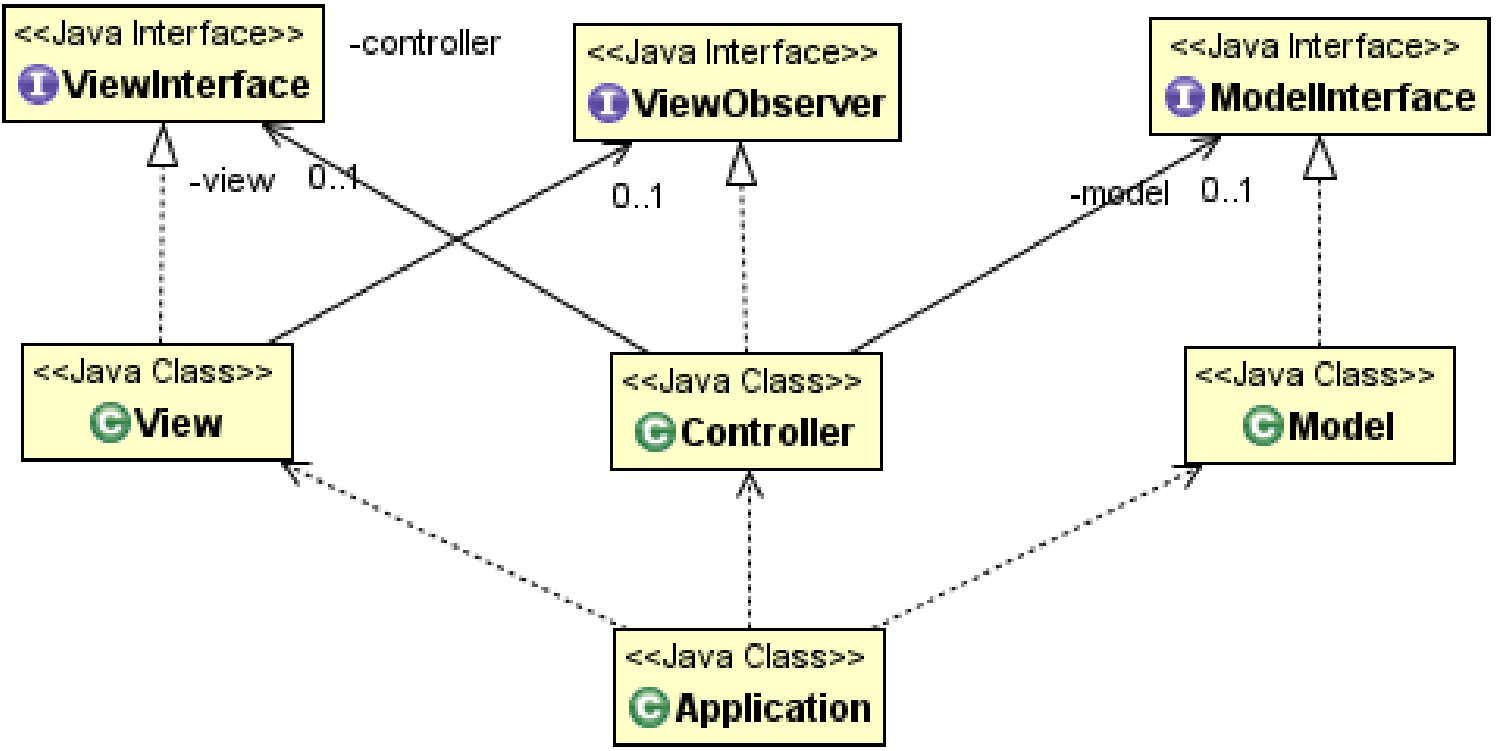
\includegraphics[scale=0.4]{img/mvc.png}
	\caption{Schema UML del pattern iniziale MVC}
	\label{img:tickingObjectTree}
\end{figure}


\section{Design dettagliato}

\subsection*{Gerarchia delle entità in gioco}

\begin{figure}[H]
	\centering{}
	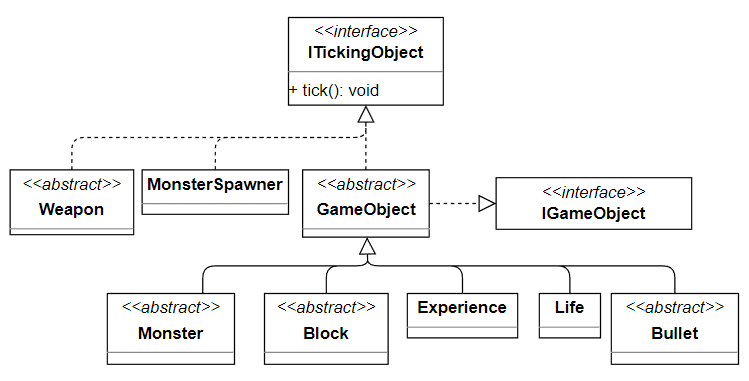
\includegraphics[width=\textwidth]{img/tickingObjectTree.png}
	\caption{Schema UML dell'organizzazione degli oggetti nel gioco}
	\label{img:tickingObjectTree}
\end{figure}

ITickingObject è l'interfaccia alla base di tutte le entità presenti in gioco, prevede il metodo tick() che permette di definire il loro comportamento ad ogni loop. Viene implementata direttamente da Weapon e MonsterSpawner in quanto sono entità che hanno bisogno di influenzare il gioco senza avere una posizione ed una texture. 

L'interfaccia IGameObject prevede tutti i metodi necessari agli oggetti di gioco con una grafica e un sistema di collisioni. 

GameObject implementa ITickingObject e IGameObject ed è la classe astratta estesa da tutte le entità di gioco che non sono puramente logiche come, ad esempio, le armi.


\subsection*{GameStatus}
\begin{figure}[H]
	\begin{center}
		\begin{tikzpicture}[scale=0.2]
			\tikzstyle{every node}+=[inner sep=0pt]
			\draw [black] (49.3,-28.5) circle (4.1);
			\draw (49.3,-28.5) node {$Running$};
			\draw [black] (37.8,-28.5) circle (4.1);
			\draw (37.8,-28.5) node {$Loading$};
			\draw [black] (21.9,-28.5) circle (4.1);
			\draw (21.9,-28.5) node {$Menu$};
			\draw [black] (65.7,-28.5) circle (4.1);
			\draw (65.7,-28.5) node {$Pause$};
			\draw [black] (49.3,-14.6) circle (4.1);
			\draw (49.3,-14.6) node {$Won$};
			\draw [black] (49.3,-42.1) circle (4.1);
			\draw (49.3,-42.1) node {$Lost$};
			\draw [black] (51.049,-24.837) arc (140.44226:39.55774:8.367);
			\fill [black] (63.95,-24.84) -- (63.83,-23.9) -- (63.06,-24.54);
			\draw [black] (63.44,-31.876) arc (-47.23207:-132.76793:8.747);
			\fill [black] (51.56,-31.88) -- (51.81,-32.79) -- (52.49,-32.05);
			\draw [black] (49.3,-24.4) -- (49.3,-18.7);
			\fill [black] (49.3,-18.7) -- (48.8,-19.5) -- (49.8,-19.5);
			\draw [black] (49.3,-32.6) -- (49.3,-38);
			\fill [black] (49.3,-38) -- (49.8,-37.2) -- (48.8,-37.2);
			\draw [black] (41.9,-28.5) -- (45.2,-28.5);
			\fill [black] (45.2,-28.5) -- (44.4,-28) -- (44.4,-29);
			\draw [black] (26,-28.5) -- (33.7,-28.5);
			\fill [black] (33.7,-28.5) -- (32.9,-28) -- (32.9,-29);
			\draw [black] (45.64,-16.45) -- (25.56,-26.65);
			\fill [black] (25.56,-26.65) -- (26.5,-26.73) -- (26.04,-25.84);
			\draw [black] (45.63,-40.28) -- (25.57,-30.32);
			\fill [black] (25.57,-30.32) -- (26.07,-31.13) -- (26.51,-30.23);
		\end{tikzpicture}
	\end{center}
	\caption{Diagramma degli stati del gioco}
\end{figure}
Per gestire gli stati nel gioco abbiamo pensato di implementare un sistema che segue un diagramma a stati finiti. Non siamo riusciti ad implementare nella sua totalità questa idea per mancanza di tempo.

\begin{itemize}
	\item \textbf{Menu}: stato all'apertura dell'applicazione e al riavvio del gioco durante il quale è visibile la schermata iniziale di gioco.
	\item \textbf{Loading}: stato durante il caricamento degli elementi di gioco.
	\item \textbf{Running}: stato durante il gioco vero e proprio, permettendo al gioco di aggiornare sia i metodi tick() che render() di tutti i GameObject.
	\item \textbf{Pause}: stato che mette il gioco in pausa, permette al gioco di aggiornare solamente il metodo render() di tutti i GameObject mettendo in pausa in metodo tick().
	\item \textbf{Won} e \textbf{Lost}: stato attivato dalla vittoria o dalla sconfitta del giocatore.
\end{itemize}

\paragraph{}
		
Si parte da una visione architetturale, il cui scopo è informare il lettore di quale sia il funzionamento dell'applicativo realizzato ad alto livello.
%
In particolare, è necessario descrivere accuratamente in che modo i componenti principali del sistema si coordinano fra loro.
%
A seguire, si dettagliano alcune parti del design, quelle maggiormente rilevanti al fine di chiarificare la logica con cui sono stati affrontati i principali aspetti dell'applicazione.

\section{Architettura}

unica interazione fra giocatore e gioco -> movimento

classe presentazione -> menu

classe motore -> loop (game) e chiama metodi dell'handler

handler

ticking automatico

rendering


Questa sezione spiega come le componenti principali del software interagiscono fra loro.
%
In particolare, qui va spiegato \textbf{se} e \textbf{come} è stato utilizzato il pattern
architetturale model-view-controller (e/o alcune sue declinazioni specifiche, come entity-control-boundary).

Se non è stato utilizzato MVC, va spiegata in maniera molto accurata l'architettura scelta, giustificandola in modo appropriato.

Se è stato scelto MVC, vanno identificate con precisione le interfacce e classi che rappresentano i punti d'ingresso per modello, view, e controller.
Raccomandiamo di sfruttare la definizione del dominio fatta in fase di analisi per capire quale sia l'entry point del model, e di non realizzare un'unica macro-interfaccia che, spesso, finisce con l'essere il prodromo ad una ``God class''.
%
Consigliamo anche di separare bene controller e model, facendo attenzione a non includere nel secondo strategie d'uso che appartengono al primo.

In questa sezione vanno descritte, per ciascun componente architetturale che ruoli ricopre (due o tre ruoli al massimo), ed in che modo interagisce (ossia, scambia informazioni) con gli altri componenti dell'architettura.
%
Raccomandiamo di porre particolare attenzione al design dell'interazione fra view e controller: se ben progettato, sostituire in blocco la view non dovrebbe causare alcuna modifica nel controller (tantomeno nel model).

\subsection*{Elementi positivi}
\begin{itemize}
	\item Si mostrano pochi, mirati schemi UML dai quali si deduce con chiarezza quali sono le parti principali del software e come interagiscono fra loro.
	\item Si mette in evidenza se e come il pattern architetturale model-view-controller è stato applicato, anche con l'uso di un UML che mostri le interfacce principali ed i rapporti fra loro.
	\item Si discute se sia semplice o meno, con l'architettura scelta, sostituire in blocco la view: in un MVC ben fatto, controller e modello non dovrebbero in alcun modo cambiare se si transitasse da una libreria grafica ad un'altra (ad esempio, da Swing a JavaFX, o viceversa).
\end{itemize}

\subsection*{Elementi negativi}
\begin{itemize}
	\item L'architettura è fatta in modo che sia impossibile riusare il modello per un software diverso che affronta lo stesso problema.
	\item L'architettura è tale che l'aggiunta di una funzionalità sul controller impatta pesantemente su view e/o modello.
	\item L'architettura è tale che la sostituzione in blocco della view impatta sul controller o, peggio ancora, sul modello.
	\item Si presentano UML caotici, difficili da leggere.
	\item Si presentano UML in cui sono mostrati elementi di dettaglio non appartenenti all'architettura, ad esempio includenti campi o con metodi che non interessano la parte di interazione fra le componenti principali del software.
	\item Si presentano schemi UML con classi (nel senso UML del termine) che ``galleggiano'' nello schema, non connesse, ossia senza relazioni con il resto degli elementi inseriti.
	\item Si presentano elementi di design di dettaglio, ad esempio tutte le classi e interfacce del modello o della view.
	\item Si discutono aspetti implementativi, ad esempio eventuali librerie usate oppure dettagli di codice.
\end{itemize}

\subsection*{Esempio}

L'architettura di GLaDOS segue il pattern architetturale MVC.
%
GLaDOS implementa l'interfaccia AI, ed è il controller del sistema.
Essendo una intelligenza artificiale, è una classe attiva.
%
GLaDOS accetta la registrazione di Input ed Output, che fanno parte della ``view'' di MVC, e sono il ``boundary'' di ECB.
Gli Input rappresentano delle nuove informazioni che vengono fornite all'IA, ad esempio delle modifiche nel valore di un sensore, oppure un comando da parte dell'operatore.
Questi input infatti forniscono eventi.
Ottenere un evento è un'operazione bloccante: chi la esegue resta in attesa di un effettivo evento.
Di fatto, quindi, GLaDOS si configura come entità \textit{reattiva}.
Ogni volta che c'è un cambio alla situazione del soggetto, GLaDOS notifica i suoi Output,
informandoli su quale sia la situazione corrente.
%
Conseguentemente, GLaDOS è un ``observable'' per Output.

\begin{figure}[h]
	\centering{}
	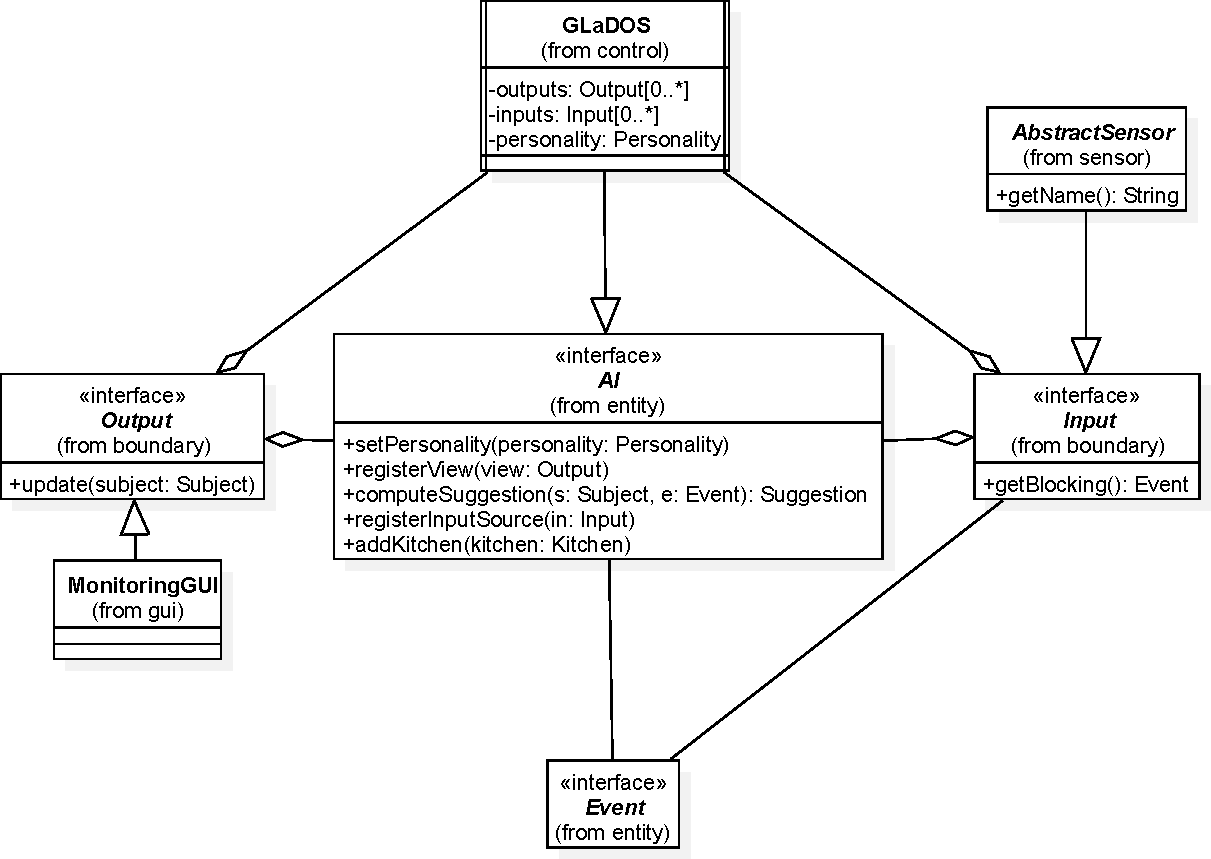
\includegraphics[width=\textwidth,scale=0.5]{img/arch}
	\caption{Schema UML architetturale di GLaDOS. L'interfaccia \texttt{GLaDOS} è il controller del sistema, mentre \texttt{Input} ed \texttt{Output} sono le interfacce che mappano la view (o, più correttamente in questo specifico esempio, il boundary). Un'eventuale interfaccia grafica interattiva dovrà implementarle entrambe.}
	\label{img:goodarch}
\end{figure}

Con questa architettura, possono essere aggiunti un numero arbitrario di input ed output
all'intelligenza artificiale.
%
Ovviamente, mentre l'aggiunta di output è semplice e non richiede alcuna modifica all'IA, la
presenza di nuovi tipi di evento richiede invece in potenza aggiunte o rifiniture a GLaDOS.
%
Questo è dovuto al fatto che nuovi Input rappresentano di fatto nuovi elementi della business
logic, la cui alterazione od espansione inevitabilmente impatta il controller del progetto.

\section{Design dettagliato}

\subsubsection*{Sergio Dobrianskiy:}
%
\begin{enumerate}

	
	\item Factory Pattern: WeaponFactory
			
	\begin{itemize}
		\item Problema: creare un'istanza delle armi presenti nel gioco durante la fase di loading indipendentemente dall'implementazione della classe astratta Weapon.
		\item Soluzione: ho deciso di usare il metodo Factory che permette di separare il codice della costruzione dell'oggetto dal codice che lo andrà ad utilizzare.
		\item Schema:
		\begin{figure}[H]
			\centering{}
			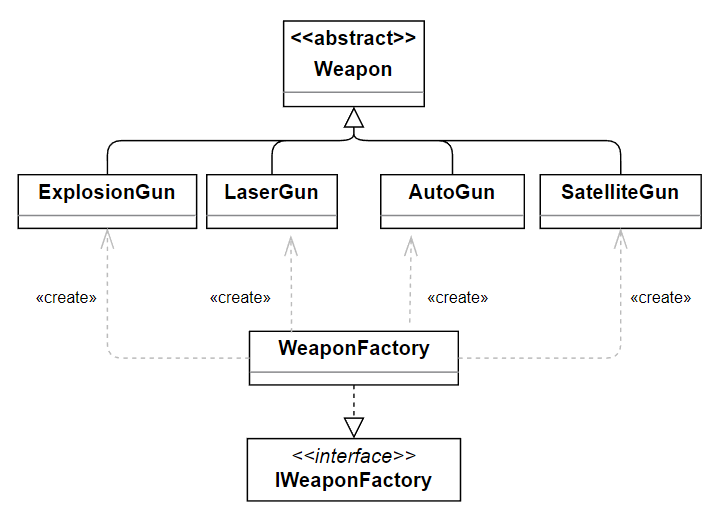
\includegraphics[width=\textwidth]{img/factory.png}
			\caption{Schema UML dell'implementazione del pattern \emph{Factory}}
			\label{img:Factory Pattern}
		\end{figure}
	\end{itemize}
	
		\item Strategy Pattern: CollisionBehavior
	\begin{itemize}
		\item Problema: gestire le collisioni dei GameObject presenti in gioco in modo efficiente 
		\item Soluzione ho deciso di usare lo Strategy Pattern che permette di definire una serie di algoritmi in classi separate e di poterli inserire in modo intercambiabile all'interno di altre classi.
		In questo modo per assegnare lo stesso comportamento a più di una classe non sarà necessario scrivere lo stesso codice più volte e rispettare il principio DRY.
		Gli algoritmi alla base di ciascun comportamento sono facilmente mantenibili e modificabili. \\
		Nella versiona attuale di gioco ho creato 3 algoritmi ciascuno gestito da una classe che implementa l'interfaccia ICollisionBehavior. 
		Un esempio dell'utilizzo di queste classi lo si può trovare nella gestione di tutte le Bullet. Di default tutte le classi che estendono la classe astratta Bullet avranno l'algoritmo NoCollisionBehavior, mentre in AutoBullet verrà usato l'algoritmo presente in RemoveOnCollisionBehavior.
		\item Schema:
		\begin{figure}[H]
			\centering{}
			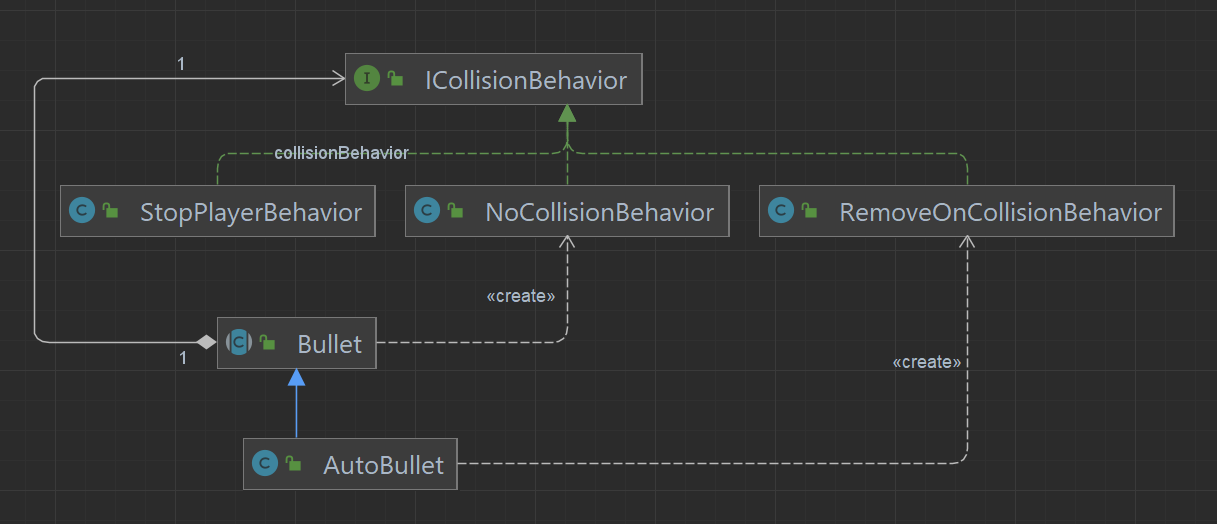
\includegraphics[width=\textwidth]{img/strategy.png}
			\caption{Schema UML dell'implementazione del pattern \emph{Strategy}. }
			\label{img:Strategy Pattern}
		\end{figure}
		
	\end{itemize}
	\item Template Method Pattern
	\begin{itemize}
		\item Problema: implementare l'algoritmo che permetta a ciascuna arma di sparare.
		\item Soluzione: ho deciso di utilizzare il Template Method in quanto il comportamento di ciascuna arma è unico e non verrà usato altrove.
		La classe astratta Weapon contiene l'algoritmo che permette alle armi che estenderanno di sparare in modo ciclico, ma il metodo che richiama lo sparo stesso è astratto e richiede di essere implementato.
		\item Schema:
		\begin{figure}[H]
			\centering{}
			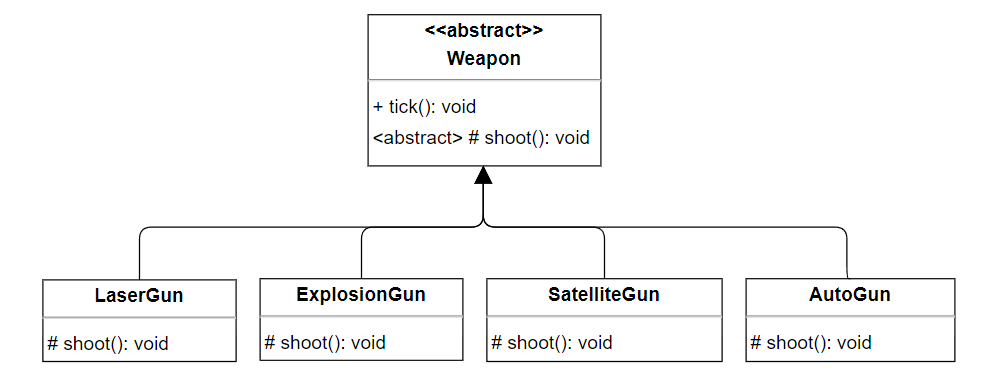
\includegraphics[width=\textwidth]{img/template.png}
			\caption{Schema UML dell'implementazione del pattern \emph{Template}}
			\label{img:Template Pattern}
		\end{figure}
	\end{itemize}
	
	
	
\end{enumerate}
%
\subsubsection*{Pierangelo Motta:}
%
\begin{enumerate}
\item Problematica: configurare metodi comuni a diversi tipi di mostri.
\begin{itemize}
	\item E' stata utilizzata la abstract class "Monster" (che implementa l'interfaccia IMonster) per definire i metodi comuni a tutte le classi che estendono la abstract class: "Triangle", "Rect", "Rhombus" e "Ball"(aggiunta in seguito).
	\\\\Nel caso di comportamenti diversi da parte di alcuni mostri rispetto ai metodi definiti nella classe astratta, si è utilizzato l'override del metodo. Ad esempio il percorso per raggiungere il player effettuato dal mostro di tipo "Ball" è disturbato da piccole variazioni.
\end{itemize}

\begin{figure}[H]
	\centering{}
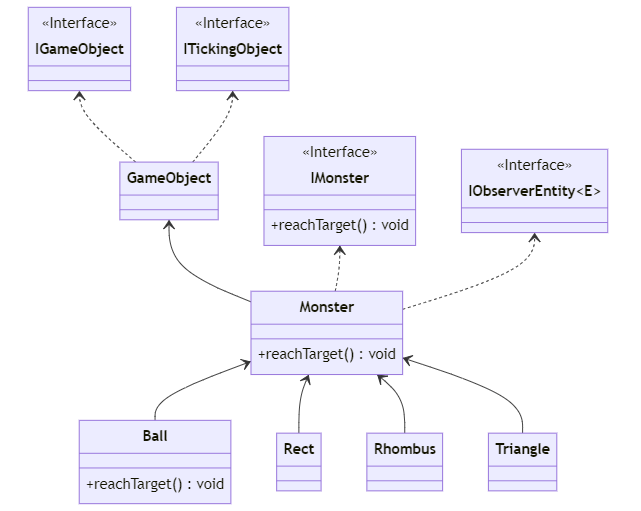
\includegraphics[width=\textwidth]{img/MonsterReachTarget.png}
	\caption{Esempio del metodo reachTarget()}
\label{img:Generate Monsters}
\end{figure}

\item Problematica: creare tipi di mostri diversi durante tutto l'arco temporale di gioco.	
\paragraph*{}
Ho utilizzato il pattern \emph{Factory Method} per avere delle factory che permettessero la creazione trasparente di mostri diversi.

La classe MonsterSpawner utilizza le factory per generare mostri diversi e con caratteristiche diverse in base allo scorrere del tempo.

\begin{figure}[H]
	\centering{}
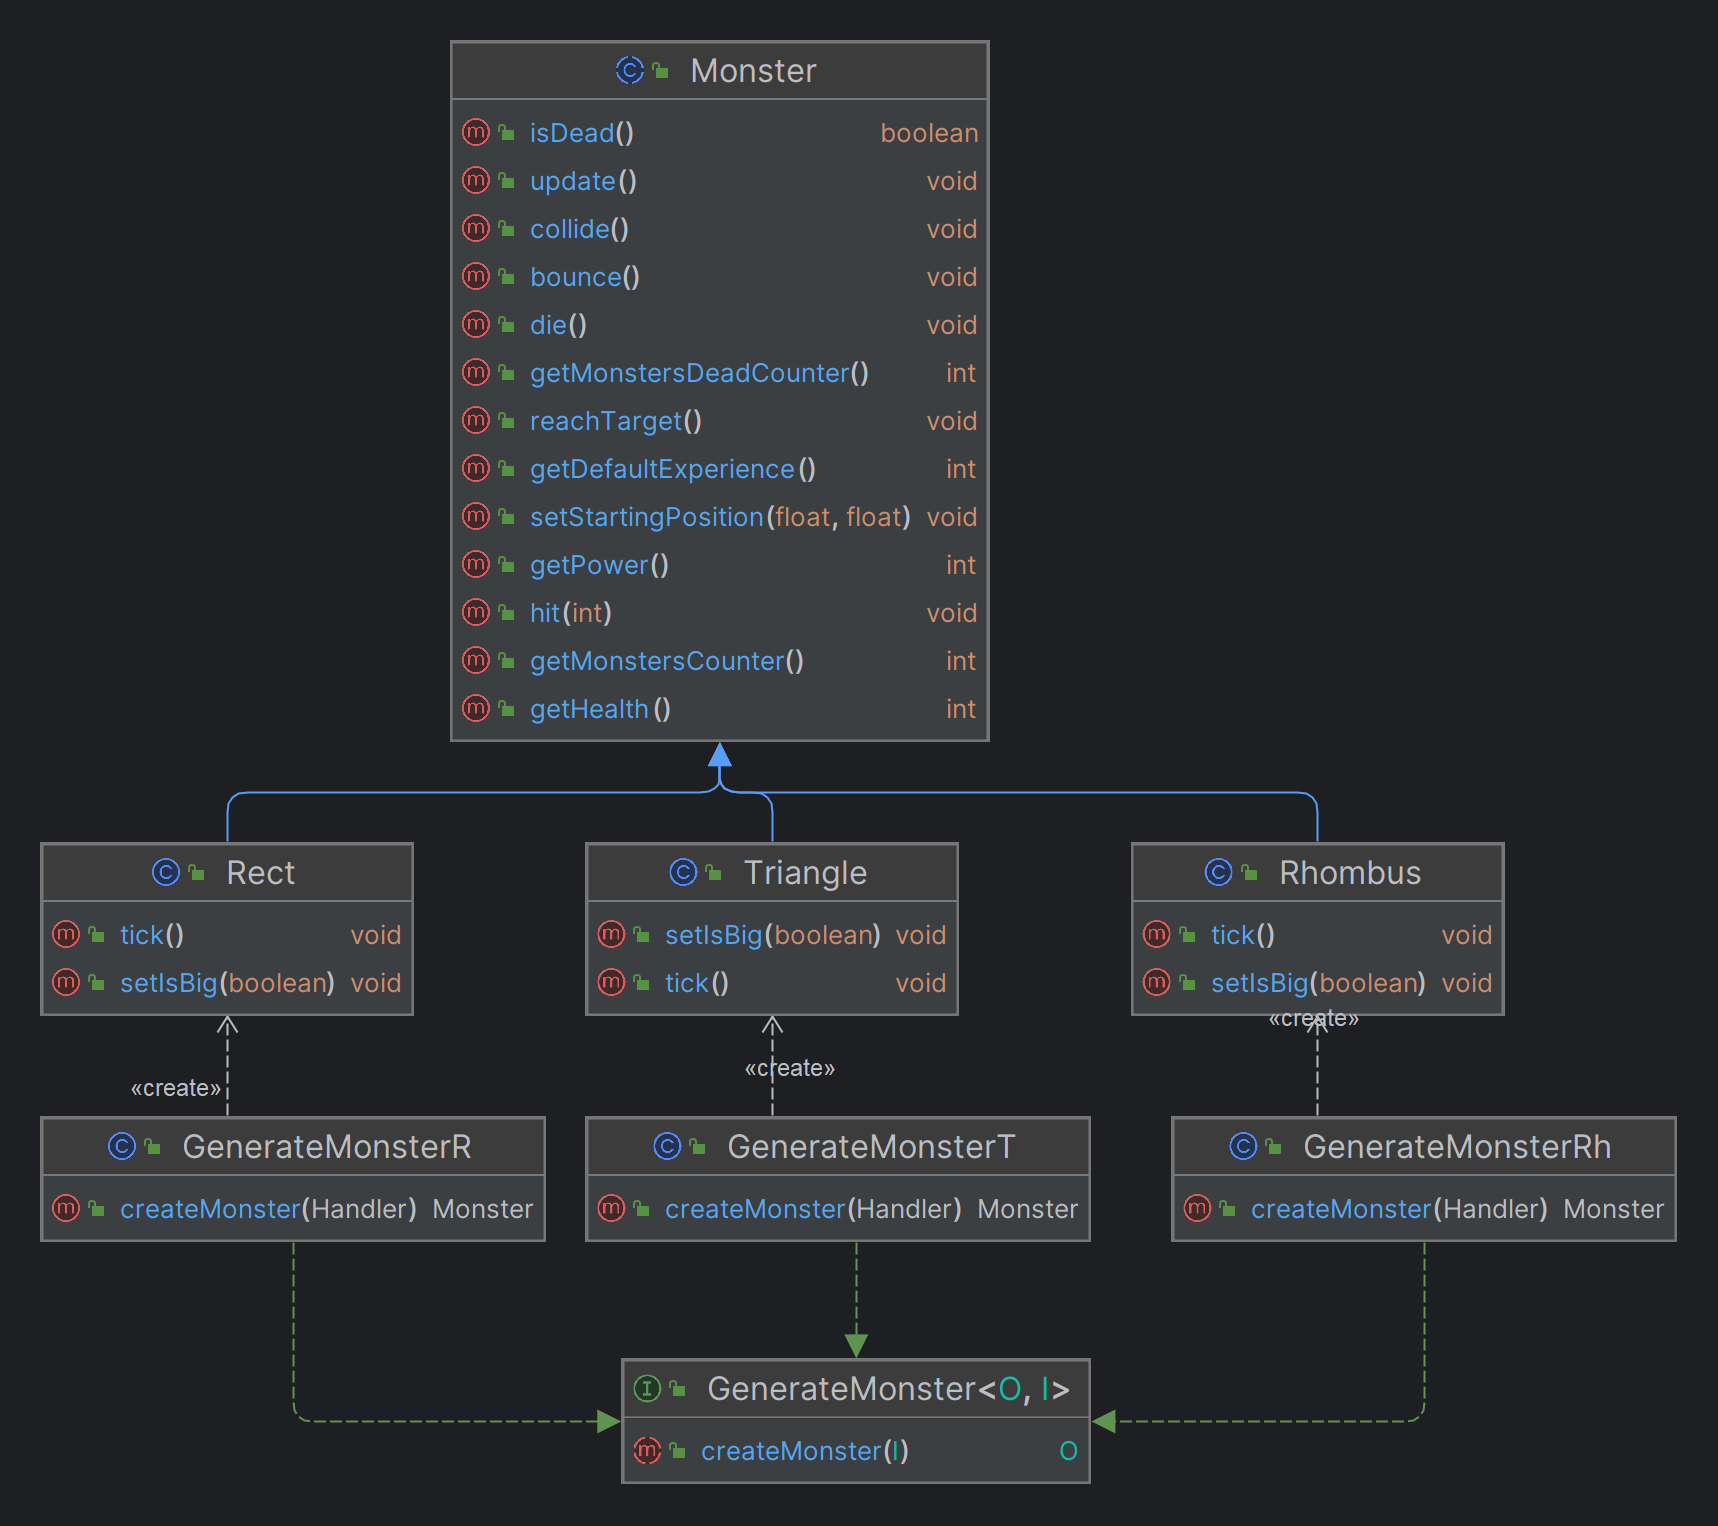
\includegraphics[width=\textwidth]{img/GenerateMonsters.png}
	\caption{Schema UML dell'implementazione, con rappresentate le entità principali ed i rapporti fra loro}
\label{img:Generate Monsters}
\end{figure}

\item Problematica: posizionare correttamente i mostri alla "nascita" e fare in modo che raggiungano il player.
%
Per la soluzione occorrono due condizioni legate dalla posizione del player nella mappa di gioco:
\begin{itemize}
	\item i mostri devono conoscere la posizione del player in ogni istante utile in quanto devono cercare di raggiungerlo per attaccarlo;
	\item i mostri devono nascere in una posizione casuale in un'area delimitata da due cerchi concentrici (di distanza minima e massima definibili) con al centro il player.
\end{itemize}
Nel primo caso ho implementato il pattern \emph{Observer}, in maniera tale che ogni mostro creato si registri in una lista di \emph{observers} del player(che è \emph{Observable}). Ad ogni tick() temporale il player \emph{notifica} tutti gli osservatori.
\paragraph{}
Ho reso generica l'interfaccia IObserverEntity \textless E\textgreater \space in maniera tale che anche altri oggetti oltre al player possano essere osservati. I metodi dell'interfaccia IObservable hanno come parametro una \emph{"bounded wildcard"} che rappresenta la possibilità di utilizzare un oggetto che appartenga ad una sottoclasse di GameObject. 
 

\begin{figure}[H]
	\centering{}
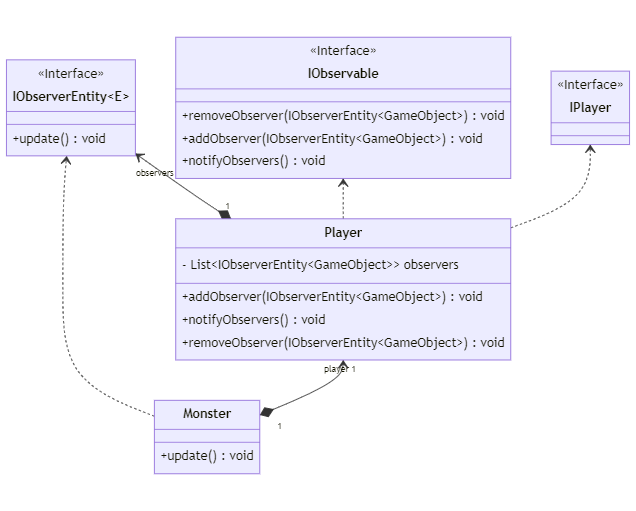
\includegraphics[width=\textwidth]{img/monsterObserver.png}
	\caption{Schema UML dell'implementazione del pattern \emph{Observer}}
\label{img:Observer Pattern}
\end{figure}

Nel secondo caso si è utilizzata una funzione di utilità Func.randomPoint() predisposta da Sergio per il calcolo delle coordinate nell'area compresa fra i due cerchi.	

\item Permettere al player di raccogliere "Experience" anche a distanza, attraverso quello che sembra una sorta di magnetismo.
\begin{itemize}
	\item Estendendo la funzionalità del punto precedente è stato possibile implementare in maniera agevole la funzionalità alla classe "Experience", in un secondo tempo, attraverso l'interfaccia IObserverEntity:
\end{itemize}
\begin{figure}[H]
	\centering{}
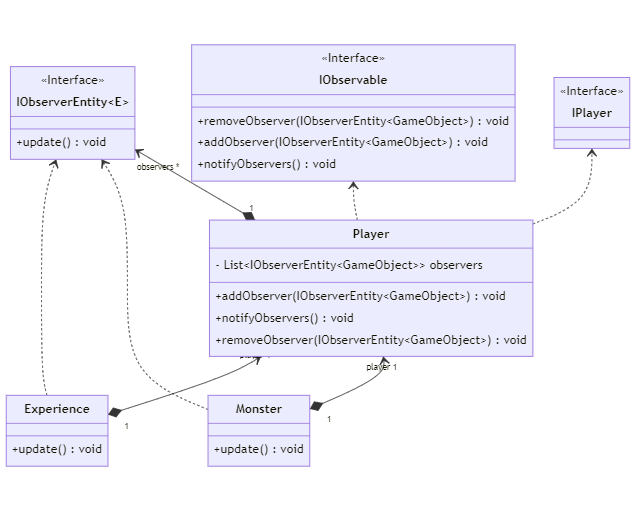
\includegraphics[width=\textwidth]{img/monsterObserver2Mermaid.png}
	\caption{Schema UML dell'implementazione del pattern \emph{Observer} per "Monster" ed "Experience"}
\label{img:Observer Pattern}
\end{figure}
%
\begin{itemize}
	\item Il metodo reachTarget() nella classe Experience è stato sovrascritto perchè il player inizia a raccogliere "pillole di esperienza" sormontandole. Con l'aumentare del livello raggiunto aumenta proporzionalmente la distanza da cui il player può raccogliere "pillole" con il solo avvicinarsi.
\end{itemize}
%
\item Problema: creare un'ondata finale di mostri per concludere il gioco.
\begin{itemize}
	\item ho creato una funzione flood() all'interno della classe MonsterSpawner) eseguita ad un certo punto temporale.
	Al suo interno, viene utilizzato uno \emph{stream} che genera un determinato tipo di mostri, fino alla fine del gioco. 
\end{itemize}
%
\item Drop di oggetti diversi alla morte di mostri
%
\begin{itemize}
	\item Alla morte di ogni mostro può essere rilascita (drop) una "pillola di esperienza", una "pillola di vita" o un nuovo mostro di tipo "Ball".
	\item La classe Drop, che implementa l'interfaccia IDrop, contiene la strategia con cui viene selezionata la tipologia di oggetto di cui fare il drop.
\end{itemize}

\item Rimbalzo del mostro colpito in movimento
%
\begin{itemize}
	\item "Effetto" grafico per emulare quanto avviene nel gioco originale, ottenuto con un semplice metodo intervenendo sulla velocità dello stesso.
\end{itemize}

\end{enumerate}
%

\subsubsection*{Thomas Testa:}
%
La mia parte di progettazione svolta riguarda:
\begin{enumerate}
    \item Player;
    \item Camera e slicing grafico;
    \item Gestione degli Input da tastiera;
\end{enumerate}

\textbf{Player}
Il Player rappresenta il personaggio principale d'ogni gioco. In questo caso la classe Player estende la classe GameObject e implementa due interfacce: IPlayer e IObservable. Sono inoltre presenti ulteriori collegamenti ad altre classi utili per lo sviluppo del giocatore all'interno del gioco. Per esempio la classe Collisions è stata utile per gestire le collisioni del Player con i mostri. E così via per le restanti classi.

\begin{figure}[H]
	\centering{}
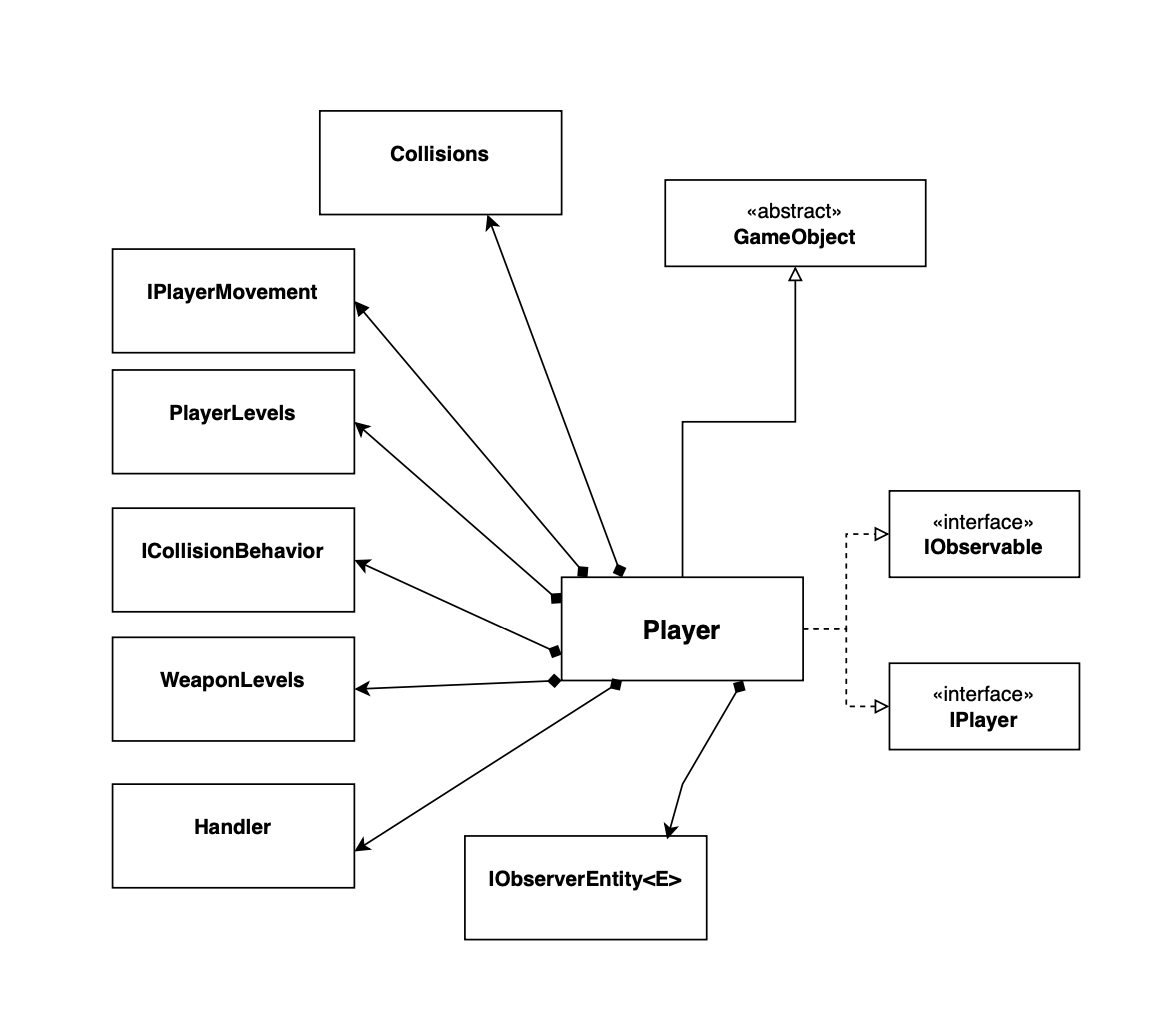
\includegraphics[width=\textwidth]{img/Player.png}
	\caption{Schema UML della classe Player}
\end{figure}

\textbf{Camera e slicing grafico}
La classe Camera rappresenta la telecamera del gioco, che segue il personaggio  durante il game. La telecamera è responsabile di mantenere il personaggio al centro dello schermo e di gestire lo spostamento della visualizzazione di quest'ultimo in base ai movimenti del giocatore.

\begin{figure}[H]
	\centering{}
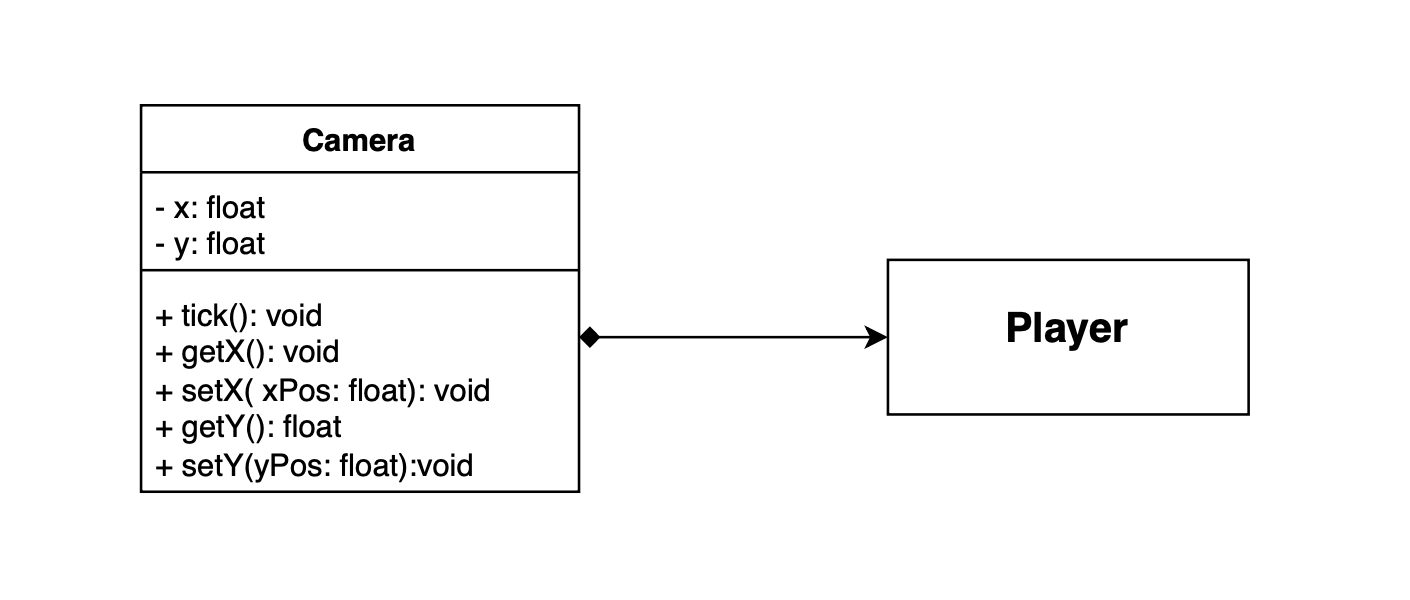
\includegraphics[width=\textwidth]{img/Camera.png}
	\caption{Schema UML della classe Camera}
\end{figure}

\textbf{Gestione degli Input}
La classe KeyInput gestisce l'input del giocatore tramite la pressione dei tasti sulla tastiera. 'KeyInput' è una sottoclasse di KeyAdapter ed estende quest'ultima per sovrascrivere i metodi keyPressed() e keyReleased() per gestire gli eventi di pressione e rilascio dei tasti. In entrambi i metodi è stato ritenuto efficiente gestire tali eventi tramite una doppia istruzione switch. Si osservi, inoltre, che i movimenti del Player sono stati gestiti sia tramite i tasti WASD sia i tasti freccia.

\begin{figure}[H]
	\centering{}
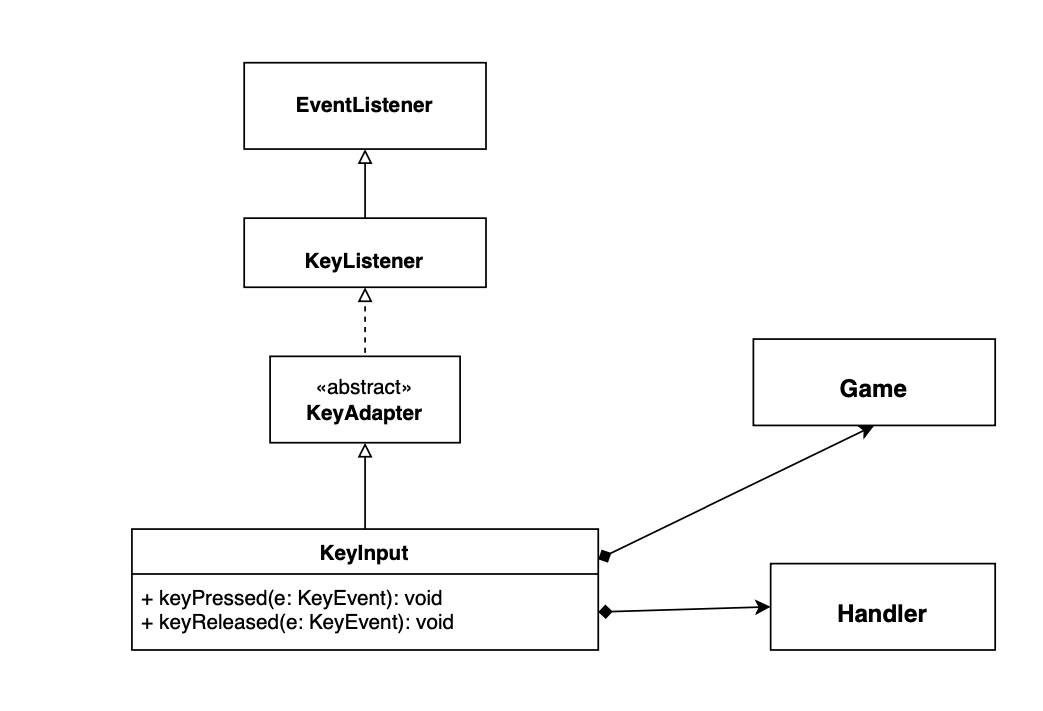
\includegraphics[width=\textwidth]{img/KeyInput.png}
	\caption{Schema UML della classe KeyInput}
\end{figure}

\begin{enumerate}
	\item Problema: Centrare la telecamera rispetto al giocatore.
	\begin{itemize}
		\item  Soluzione: la posizione della camera viene aggiornata in modo che segua il giocatore. Questo viene fatto calcolando la differenza tra la posizione del giocatore ('tempPlayer.getX()' e 'tempPlayer.getY()') e la posizione desiderata della telecamera (metà della larghezza e altezza della finestra di gioco). 
		Inoltre è stato applicato un fattore di interpolazione ('0.05f' nel codice fornito) per ottenere un movimento quanto più possibile  fluido.
	\end{itemize}
	\item Problema: Gestire la telecamera ai bordi della mappa di gioco.
	\begin{itemize}
		\item Soluzione: sono stati creati dei controlli che limitano la posizione della telecamera all'interno dei limiti definiti. 
		Ad esempio, se la posizione 'x' della telecamera è inferiore a '0', viene impostata a '0' per evitare che la telecamera esca oltre il bordo sinistro del livello di gioco. Lo stesso viene fatto per i limiti superiori ('1045' per 'x' e '1500' per 'y' nel codice fornito).
	\end{itemize}
	\item Problema: gestire la pressione di due tasti per il movimento del Player premuti contemporaneamente.
	\begin{itemize}
		\item  Soluzione:la classe Handler tiene traccia dello stato dei tasti premuti tramite le variabili booleane 'up', 'down', 'left' e 'right' e poi le singole classi degli oggetti del gioco utilizzano tali informazioni per gestire l'input e l'interazione del giocatore.
	\end{itemize}
\end{enumerate}
%


\chapter{Sviluppo}
\section{Testing automatizzato}

Pierangelo Motta:
\begin{itemize}
	\item settaggio ambiente di test Junit
	\item TestMonsterCreation: per verificare la creazione di tipi diversi di entità utilizzando le factory
	\item TestMonsterCreation: per verificare l'esistenza dei mostri attraverso il corretto conteggio degli stessi
	\item TestMonsterDie: verifica in step successivi della presenza nel gioco del "Player" e di un numero N di mostri. Alla morte di tutti i mostri verifica della presenza delle altre possibili tipologie di entità nate di conseguenza: "Experience", "Life" oppure "Ball" (mostro zombie).
\end{itemize}
%
Sergio Dobrianskiy:
\begin{itemize}
	\item TestBullets: per verificare la creazione e il corretto funzionamento delle 4 classi che estendono Bullet.
	\item TestWeapons: per verificare la creazione e il corretto funzionamento delle 4 classi che estendono Weapon.
	\item TestCollisions: per verificare la creazione e il corretto funzionamento della meccanica di collisione tra vari GameObject. Assicura anche che elementi come AutoBullet vengano rimossi dopo che è accaduta una collisione, mentre elementi come Satellite rimangano in gioco.
\end{itemize}
%
Thomas Testa:
\begin{itemize}
	\item TestPlayer: I test verificano il comportamento dei metodi della classe Player attraverso una serie di asserzioni.
	\\Nel primo test, annotato con @Test, viene verificato che il valore iniziale dell'esperienza del giocatore sia 0. Viene chiamato il metodo getExperience() dell'oggetto player e il suo valore viene confrontato con l'expectedExperience (che è 0) utilizzando l'asserzione assertEquals(). Se i valori sono diversi, il test fallisce.
    \\Nel secondo test, viene verificato che il livello iniziale del giocatore sia 1. Il processo è simile al primo test, ma viene utilizzato il metodo getLevel() invece di getExperience().
    \\Nel terzo test, viene verificato che il valore iniziale della vita del giocatore sia 100. Il processo è simile ai test precedenti, ma viene utilizzato il metodo getLife().
    \\Nel quarto test, viene testato il metodo hit(). Viene inflitto un danno di 50 al giocatore utilizzando il metodo hit(), quindi si verifica che la vita del giocatore sia diminuita a 50. Questo viene fatto confrontando il valore attuale della vita del giocatore con l'expectedLife.
    \\Nel quinto test, viene testato il metodo setLife(). Viene impostata una vita negativa (-50) per il giocatore utilizzando il metodo setLife(). Tuttavia, la vita del giocatore non può essere inferiore a 0, quindi ci si aspetta che la vita effettiva sia ancora 50. Viene confrontato l'expectedLife con il valore attuale della vita del giocatore.
\end{itemize}

\section{Metodologia di lavoro}
Il gruppo ha lavorato in modo coeso sia durante la scelta del tipo di progetto da realizzare che successivamente per la stesura di una lista di funzionalità minime da portare a termine. Ciascun membro ha scelto da questa lista le parti sulle quali avrebbe lavorato. Fatto ciò, sempre in gruppo, abbiamo deciso un design architetturale da seguire. 

Lungo il corso di tutto il progetto sono stati utilizzati un gruppo Whatsapp per la comunicazione quotidiana, un canale Discord per le riunioni settimanali e un documento condiviso su Google Drive per appunti e materiale utile. Dato che i membri del gruppo vivono lontani tra di loro e almeno due sono lavoratori full time non è stato possibile organizzare incontri dal vivo. 

Lavorando al progetto ci siamo resi conto che il modello architetturale previsto nelle prime fasi era inadeguato. Questo problema è stato risolto grazie alla comunicazione frequente tra i membri. 

Un'ulteriore difficotà è nata a causa di problemi personali del collega Matteo Trezza che, nonostante i tentativi di aiuto, ha faticato a stare al passo con il resto del gruppo e alla fine ha dovuto ritirarsi. Dato il bisogno di portare avanti le parti di Matteo, in sua assenza abbiamo provveduto a spartircele in base alle necessità e preferenze di ciascuno dei membri rimanenti.

Per condividere il codice è stato usato fin da subito Git. Ci siamo impegnati a non lavorare direttamente sul branch \textit{master} e a creare per ciascuna feature un branch separato. Per consentire a tutti di avere un codice aggiornato abbiamo cercato di fare dei merge frequenti.

Di seguito è indicata nel dettaglio la suddivisione dei compiti:

\subsection*{Sergio Dobrianskiy:}
\begin{itemize}
	\item Impostazione e supporto ai colleghi relativamente al software "Git" ed al repository "GitHub"
	\item Gestione delle armi e dei proiettili
	\item Gestione delle collisioni (tramite funzioni geometriche di java.awt)
	\item Architettura dei GameObject e TickingObject
	\item Gestione caricamento e loop di gioco (Loader e Handler)
	\item Gestione delle texture/sprite
	
	Inizialmente avevo scelto di occuparmi solo delle armi, dei proiettili e delle collisioni, ma data la necessità e l'interesse personale ho finito per occuparmi in modo massiccio anche degli altri punti indicati nella lista. 
	
	Per la gestione delle collisioni ho utilizzato le funzioni geometriche presenti in \textit{java.awt}.
	
	Come indicato nella sezione apposita, ho preso spunto dal codice del progetto "OOP21-ciccio-pier" per la creazione della classe Texture e la gestione degli sprite.
\end{itemize}
\paragraph{}

\subsection*{Pierangelo Motta:}
\begin{itemize}
	\item Impostazione e supporto ai colleghi per la parte di configurazione/utilizzo del tool "Gradle"
	\item Supporto per la verifica dei warning/errori indicati dai tool "PMD", "SpotBugs" e "CheckStyle", con correzione di diverse segnalazioni 
	\item Impostazione per la parte di configurazione/utilizzo di test Junit
	\item Gestione delle "Drop"
	\item Gestione informazioni di debug
	\item Creazione e gestione delle tipologie di entità: "mostri", "pillole di vita" ed "esperienza"
	\item Interventi in classi di altri colleghi per la gestione della vita e dell'esperienza del player e delle collisioni fra armi e "mostri"
	
	Il confronto con Sergio per la parte relativa alle collisioni fra le entità è stato continuo.

\end{itemize}
\subsection*{Thomas Testa:}
\begin{itemize}
	\item Creazione e gestione Menù 
    \item Creazione e gestione del Player (incluso i suoi movimenti)
	\item Gestione degli input da tastiera per il movimento del Player 
    \item Creazione classe Camera
    \item Gestione dello slicing grafico della telecamera
    \item Creazione mappa di gioco
\end{itemize}

\paragraph{}


\section{Note di sviluppo}

Per facilitarci nello sviluppo del gioco, soprattutto nelle fasi iniziali, abbiamo seguito dei tutorial oppure sono state usate delle funzionalità di un altro progetto, di seguito viene fortina una lista:
\begin{itemize}
	\item Per la creazione da zero del motore di gioco e del motore grafico abbiamo preso spunto da due tutorial presenti su Youtube: 
	 \begin{itemize}
	 	\item \href{https://www.youtube.com/playlist?list=PLWms45O3n--5vDnNd6aiu1CSWX3JlCU1n}{Java Game Programming Wizard Course}
	 	\item \href{https://www.youtube.com/playlist?list=PLWms45O3n--5vv69_AlMw23O1Z31CaW1F}{Java Programming Let's Build a Zombie Game}
	 \end{itemize}
	 In particolare con l'aiuto di questi due tutorial sono state poste le basi delle classi Game, GameObject, Handler, KeyInput usate per ottenere una versione rudimentale del motore di gioco e del suo motore grafico.
	 Da quel momento in poi le classi sono state fortemente riviste nelle funzionalità e riadattate ad una logica OOP.
	 
	 \item Per il caricamento e la gestione delle texture/sprite che avviene in particolare nelle classi Texture e Loader e la creazione di Block durante il cariamento della mappa è stato preso e riadattato del codice dal progetto 
	 \href{https://github.com/Valdi1111/OOP21-ciccio-pier}{OOP21-ciccio-pier} consegnato da un altro gruppo per l'esame di Programmazione ad Oggetti.
	 
\end{itemize}

\paragraph{}

\subsection{Note di sviluppo}

\subsubsection{Sergio Dobrianskiy}
Funzionalità avanzate utilizzate:
 \begin{itemize}
 	\item Utilizzo di Lambda e Stream
 	 \begin{itemize}
 	 	\item Permalink: \url{https://github.com/Sergio-Dobrianskiy/OOP22-geo-surv/blob/1d19887356d83d29b39fe301273ba64ba44ce662/src/main/java/it/unibo/geosurv/model/collisions/Collisions.java#LL33C9-L51C12}
 	 	\item Permalink: \url{https://github.com/Sergio-Dobrianskiy/OOP22-geo-surv/blob/5962bab31e3fd7033c2b8bd0e84b13aa7f7c85ef/src/main/java/it/unibo/geosurv/model/Handler.java#LL35C6-L35C6}
 	 \end{itemize}
 	 
 	 \item Utilizzo Optional
 	 \begin{itemize}
 	 	\item Permalink: \url{https://github.com/Sergio-Dobrianskiy/OOP22-geo-surv/blob/90872064704901ac999cb7efdd65f191599eefa4/src/main/java/it/unibo/geosurv/control/weapons/WeaponFactory.java#L29}
 	 \end{itemize}
 	 
 	 \item Sviluppo di algoritmi di utility per il progetto, in particolare quello che restituisce un punto random in un cerchio o in un anello attorno a un punto
 	 \begin{itemize}
 	 	\item Permalink: \url{https://github.com/Sergio-Dobrianskiy/OOP22-geo-surv/blob/90872064704901ac999cb7efdd65f191599eefa4/src/main/java/it/unibo/geosurv/model/utility/Func.java#LL32C1-L32C1}
 	 \end{itemize}
 	 
	\item Utilizzo di java.awt e java.awt.geom per la gestione delle collisisoni
 	 \begin{itemize}
 	 	\item Permalink: \url{https://github.com/Sergio-Dobrianskiy/OOP22-geo-surv/blob/90872064704901ac999cb7efdd65f191599eefa4/src/main/java/it/unibo/geosurv/model/GameObject.java#L207}
 	 	\item Permalink: \url{https://github.com/Sergio-Dobrianskiy/OOP22-geo-surv/blob/90872064704901ac999cb7efdd65f191599eefa4/src/main/java/it/unibo/geosurv/model/collisions/Collisions.java#LL84C7-L84C7}
 	 \end{itemize}
\end{itemize}

\subsubsection{Pierangelo Motta}
Funzionalità avanzate utilizzate:
 \begin{itemize}
 	\item Utilizzo di Stream
 	 \begin{itemize}
 	 	\item Permalink: \url{https://github.com/Sergio-Dobrianskiy/OOP22-geo-surv/blob/2272bc0e95fbd9f3b223109b6c7b9012c63c97f2/src/main/java/it/unibo/geosurv/model/monsters/MonsterSpawner.java#LL116C1-L121C20}
 	 \end{itemize}
 	 
 	\item Utilizzo di generici
 	 \begin{itemize}
 	 	\item Permalink: \url{https://github.com/Sergio-Dobrianskiy/OOP22-geo-surv/blob/2272bc0e95fbd9f3b223109b6c7b9012c63c97f2/src/main/java/it/unibo/geosurv/model/drops/IDrop.java#LL1C1-L15C2}
 	 	\item Permalink: \url{https://github.com/Sergio-Dobrianskiy/OOP22-geo-surv/blob/2272bc0e95fbd9f3b223109b6c7b9012c63c97f2/src/main/java/it/unibo/geosurv/model/monsters/GenerateMonster.java#L10}
 	 	 	 	\item Permalink: \url{https://github.com/Sergio-Dobrianskiy/OOP22-geo-surv/blob/2272bc0e95fbd9f3b223109b6c7b9012c63c97f2/src/main/java/it/unibo/geosurv/model/IObserverEntity.java#LL8C1-L8C37}
 	 \end{itemize}
	\item Utilizzo di Wildcard (upper bound)
 	\begin{itemize}
 	 	\item Permalink: \url{https://github.com/Sergio-Dobrianskiy/OOP22-geo-surv/blob/2272bc0e95fbd9f3b223109b6c7b9012c63c97f2/src/main/java/it/unibo/geosurv/model/IObservable.java#L13}
 	\end{itemize}
 	\begin{itemize}
 	 	\item Permalink: \url{https://github.com/Sergio-Dobrianskiy/OOP22-geo-surv/blob/2272bc0e95fbd9f3b223109b6c7b9012c63c97f2/src/main/java/it/unibo/geosurv/model/IObservable.java#L20}
 	\end{itemize}
	
\end{itemize}






\chapter{Commenti finali}

\section{Autovalutazione e lavori futuri}
\subsubsection*{Sergio Dobrianskiy:}

Ho  cercato i membri per formare il gruppo e proposto l'idea di gioco sulla quale lavorare.
Durante lo svolgimento del progetto ho cercato di indirizzare ciascun membro su obbiettivi a breve termine che mi sembravano più importanti, in particolar modo durante le fasi iniziali ho insistito sulle funzionalità necessarie a tutto gruppo per poter procedere nello sviluppo. 
Quando mi sono reso conto che il collega Matteo Trezza non avrebbe portato a termine la sua parte di progetto mi sono occupato di una buona parte delle sue funzionalità minime.

Sono soddisfatto del lavoro fatto da me e dal gruppo, l'organizzazione e il team work sono stati ottimi. Inoltre creare da zero un gioco, anche se semplice, mi ha appassionato e mi ha permesso di imparare molto.
Il mio punto debole è stata la totale inesperienza con lo sviluppo di un gioco che mi ha reso impossibile avere un'idea chiara sulla scaletta di cosa sviluppare nel medio-lungo periodo. Inoltre la scarsa famigliarità iniziale con i pattern di programmazione mi hanno costretto a un refactoring in corso d'opera. 

Se dovessi continuare a lavorare al progetto vorrei lavorare su una versione mobile e riscrivere in modo migliore la parte del motore di gioco.

\subsubsection*{Pierangelo Motta:}

La sfida è stata interessante perchè l'ambito è completamente al di fuori degli interessi personali e di quello a cui sono abituato lavorativamente parlando.

Ho cercato di supportare i membri del gruppo in alcuni passaggi di carattere generale risolvendo alcune problematiche di tipo, diciamo, sistemistico.

Cosi come Sergio, anche io ho sperimentato una fase iniziale di difficoltà nell'analisi e progettazione senza avere la visione completa dei vari passaggi e delle eventuali problematiche pratiche di implementazione. Questo a portato a diverse modifiche nel corso del tempo.

Un punto di debolezza personale è non essere riuscito ad implementare codice utilizzando un approccio di tipo "funzionale".

\subsubsection*{Thomas Testa:}

Il progetto è stato molto stimolante. Era la prima volta che partecipavo alla creazione di un videogioco.

Questo progetto mi ha permesso di ampliare le mie conoscenze riguardanti la programmazione ad oggetti, soprattutto grazie anche alla collaborazione con i componenti del mio gruppo Sergio e Pierangelo in quanto sono stati di ottimo supporto per far fronte a qualsiasi tipo di problematica riscontrata durante questa avventura. 

Sono soddisfatto del lavoro fatto. Personalmente, per il codice scritto da me, avrei potuto far utilizzo di pattern o espressioni che avrebbero migliorato la qualità del codice. Sono sicuro che sotto questo punto di vista, quest'esperienza si rivelerà molto utile per eventuali progetti futuri non solo di questo genere.
\paragraph{}

\appendix
\chapter{Guida utente}

%{\color{red}Credo si possa eliminare visto la schermata menu di gioco}
Il player deve sfuggire ai mostri muovendosi con le le frecce direzionali o con i comuni tasti W (su) A(sinistra) S(giù) D(destra).
\paragraph{}
Il player inizia il gioco con un'arma a disposizione e, all'aumentare di livello, vengono aggiunte nuove armi e tutte si potenziano.
%
Il livello cresce se il player raccoglie gemme blu ("pillole di esperienza") create dalla morte dei mostri.
Alla morte di un mostro potrebbero anche essere rilasciati una gemma verde("Life") che se raccolta fornisce un recupero di vita al player oppure potrebbe essere creato un nuovo tipo di mostro("Ball").
\paragraph{}
Il gioco finisce se il player esauriusce la vita a disposizione (il player muore) o dopo un minuto di gioco, soppravivendo all'arrivo di un'ondata finale di mostri (il player vince).
\paragraph{}
Come indicato nella schermata iniziale:
\begin{itemize}
\item p) mette il gioco in pausa;
\item g) attiva la modalità di debug che mostra informazioni sugli oggetti presenti.
\end{itemize}


% \bibliographystyle{alpha}
% \bibliography{13-template}

\end{document}
